\chapter{ESPECIFICAÇÃO DO PROJETO} % (fold)
\label{cha:especificacao_do_projeto}

 O projeto consiste no desenvolvimento de um sistema de recomendação acoplado a uma rede social. As recomendações realizadas pelo sistema serão baseadas em similaridade de itens, em similiradade de perfil e na confiança implícita entre os usuários.

\section{Visão Geral do Sistema} % (fold)
\label{sec:visao_do_sistema}

O sistema de recomendação utilizará a rede social para obter as relações de amizade entre usuários. Esta relação é estabelicida entre dois usuários após ambos a confirmarem através do envio de um convite de amizade ou da aceitação deste.

Os usuários podem avaliar produtos (previamente cadastrados na base de dados) e receber recomendações de outras pessoas presentes na rede social. Tendo como base o comportamento do usuários nestas atividades o sistema será capaz de enviar novas recomendações de produtos relevantes ao usuário.

 Os principais blocos do sistemas podem ser vistos na Figura~\ref{fig:escopo}. A rede social é utilizada para o estabelecimento das relações de amizade, para a criação e visualização de avaliações dos produtos e para o envio de recomendações. O reposotório é utilizado armezenar os produtos cadastrados e as recomendações a serem enviadas. Já o sistema de recomendação tem o papel de analisar as informações contidas no repositório e gerar novas recomendações.

\begin{figure}
  \centering
  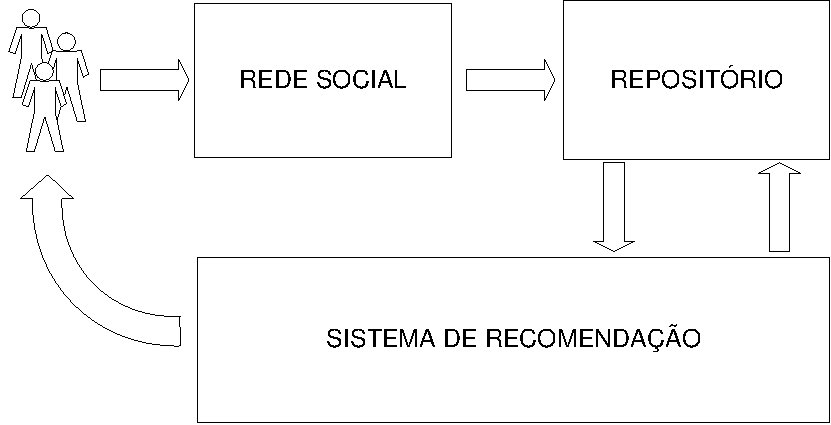
\includegraphics[width=\textwidth]{imagens/Diagrama_Visao_Geral}
  \caption{\it Diagrama de blocos do sistema}
  \label{fig:escopo}
\end{figure}

% section visao_do_sistema (end)

\section{Descrição do Sistema}

 Através do sistema os usuários poderão indicar o interesse em produtos e realizar recomendações a outros usuários. Quando um usuário avaliar um produto recomendado por outro usuário o índice de confiança deste em relação ao outro é ataulizado no sistema. Com base nas recomendações e nas avaliações o sistema irá inferir as seguintes informações:
 
\begin{itemize}

 \item Similaridade entre usuários

 \item Similaridade entre produtos

 \item Grau de confiança entre usuários

 \item Recomendações de produtos mais relevantes para um determinado usuário

\end{itemize}

 Para a obtenção das recomendações será feito um experimento para determinar quais critérios inferidos são mais importantes de forma que o sistema apresente uma boa acurácia, abrangência e alta satisfação dos usuários. As recomendações geradas pelo sistema são baseadas na similiraridade entre as avaliações feitas pelos usuários, nas relações de confiança, e nas relações encontradas entre os produtos.

  O usuário do sistema tem a opção de buscar produtos já cadastrados. Além disso, os usuários podem recomendar os produtos para outros usuários presentes na rede social. Os usuários serão instruídos a direcionadar as recomendações para as pessoas que provavelmente gostariam do produto.

 Ao receber uma recomendação o usuário é instruído a avaliar o produto recomendado para que o sistema atualize as informações relativas aos seus interesses. Estas informações são utilizadas para verificar a similaridade entre usuários, a similaridade entre itens e o índice de confiança.
 
 Quando um usuário avalia um produto recomendado por outro, essa avaliação altera o grau de confiança do usuário que recomendou o produto em relação àquele que recebeu a recomendação. Caso a avaliação seja positiva, a confiança do receptor aumenta, porém, caso a avaliação seja negativo, significa que o usuário que recebeu a recomendação não a aceitou como relevante, diminuindo o índice de confiança.

 O sistema armazena as informações referentes as avaliações de produtos e os índices de confiança entre usuários. Essas informações são utilzadas para sugerir outros produtos que os usuários possam gostar. Esse é um dos propósitos do sistema de recomendação: mostrar ao usuário apenas informações relevantes.

\section{Funcionalidades principais} % (fold)
\label{sec:funcionalidades_principais}

Abaixo estão sumarizadas as principais funcionalidades do sistema acompanhadas das descrições em formato de \textit{user stories}\cite{557458}:

\begin{itemize}
	
	\item Avaliação de produto
  \subitem Como usuário, quero fazer a minha avaliação de produtos para que outros tenham conhecimento da minha opinião.
  
	\item Recomendação de produtos baseada em preferência do usuário
	\subitem Como usuário, eu quero receber uma lista de produtos que eu provavelemente goste para que eu não precise filtrar os itens que me interessam.

	\item Envio de recomendação de produto a outro usuário
  \subitem Como recomendador, quero enviar uma recomendação de produto para outra pessoa para que ela conheça a minha opinião sobre este item.

    \item Visualização das avaliações recentes dos amigos
    \subitem Como usuário, quero estar ciente sobre as últimas avaliações dos meus amigos para que eu possa saber o que acontece no meu contexto social e conheça novos produtos.

    \item Feedback de recomendação
    \subitem Como recomendador, quero receber feedback sobre as recomendações que enviei para me incentivar a fazer melhores recomendações.
	
\end{itemize}

\section{Requisitos não-funcionais}

Os principais requisitos não-funcionais do sistema são:

\begin{itemize}

    \item Interface web compatível as últimas versões dos \textit{browsers} Internet Explorer, Mozilla Firefox e Safari.
    
    \item \textit{Backend} compatível com servidores Linux.

    \item Tempo médio de resposta menor que 2 segundos para 10 usuários simultâneos quando executado em um servidor com processador Intel Core 2 Duo T7250 ou superior e 2 GB de memória RAM. % esta é a configuração do meu notebook -- Allan

\end{itemize}

\section{Limites do Sistema}

\begin{itemize}
  
    \item O sistema não fará processamento de linguagem natural\footnote{\textit{Natural Language Processing (NLP)}}

\end{itemize}

\section{Implementação} % (fold)
\label{sec:implementacao}


% section implementacao (end)

% chapter especificacao_do_projeto (end)
